% vim:set spell:
% vim:spell spelllang=fr:
\documentclass[a4paper]{article}
\usepackage[utf8x]{inputenc}
\usepackage[T1]{fontenc}
\usepackage{charter}
\usepackage{graphicx}
\usepackage{amsmath,amssymb}
\usepackage[french]{babel}
\usepackage{xspace}
\usepackage{setspace}
\setstretch{1.0}
\usepackage{subfigure}
\usepackage{listings}
\voffset       -1in
\hoffset       -1in
\headheight     12pt
\headsep        12pt
\topmargin      25mm
\oddsidemargin  20mm
\textwidth      170mm
\textheight     240mm
\flushbottom
\lstset{numbers=left, numberstyle=\tiny, stepnumber=1, numbersep=5pt}
\graphicspath{{../../scripts/}}
\begin{document}
\begin{center}
    \large
    Travaux Pratiques Archi ISI-3A\\
    \LARGE
    Prédiction de branchements\\
    \large
\end{center}

\section{Identification}
    Travail réalisé par Lalie Arnoud et Quentin Blasiak

\section{Prédicteur $n$ modal : conception et résultats}
    \subsection{Conception}
    Le prédicteur $n$ modal bit est constitué d'un unique tableau contenant de $2^1$ à $2^3$ bits.

    \subsection{Résultats}
    Les résultats issus de la simulation sont les suivants.
    \par
    \begin{minipage}{.48\linewidth}
    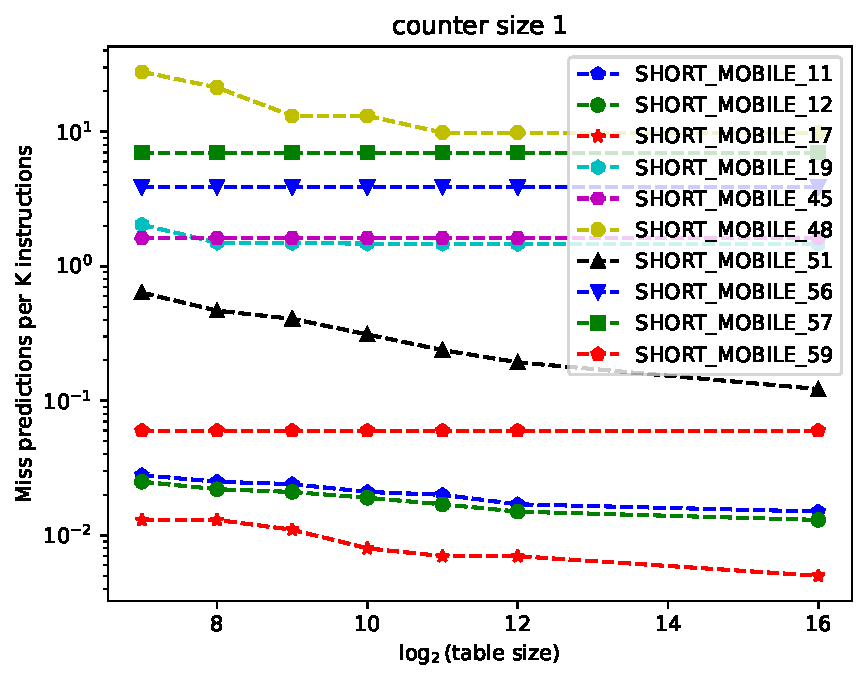
\includegraphics[width=\linewidth]{modal/graph_1_modal}
    \end{minipage}%
    \hfill
    \begin{minipage}{.48\linewidth}
    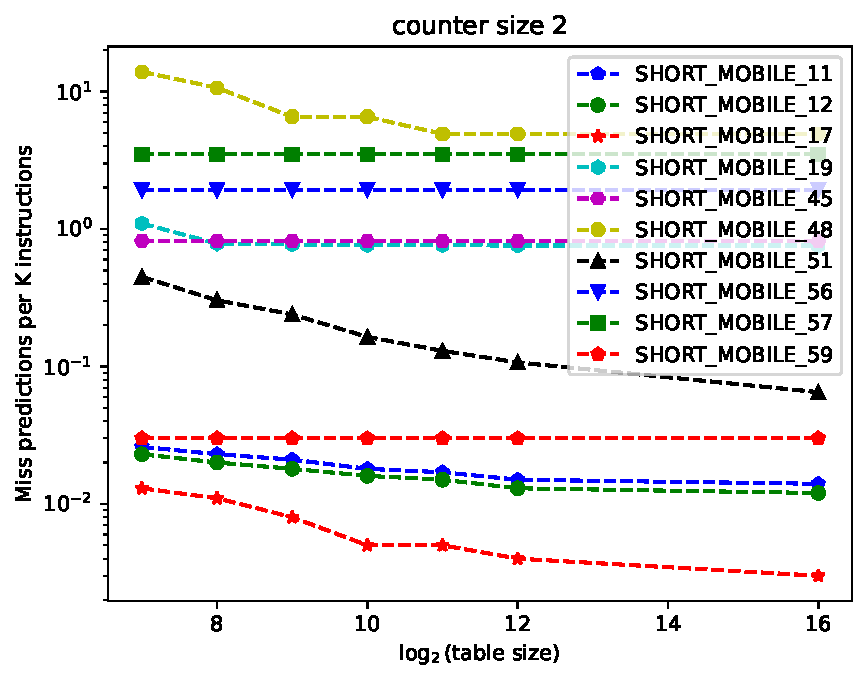
\includegraphics[width=\linewidth]{modal/graph_2_modal}
    \end{minipage}

    \begin{minipage}{.48\linewidth}
    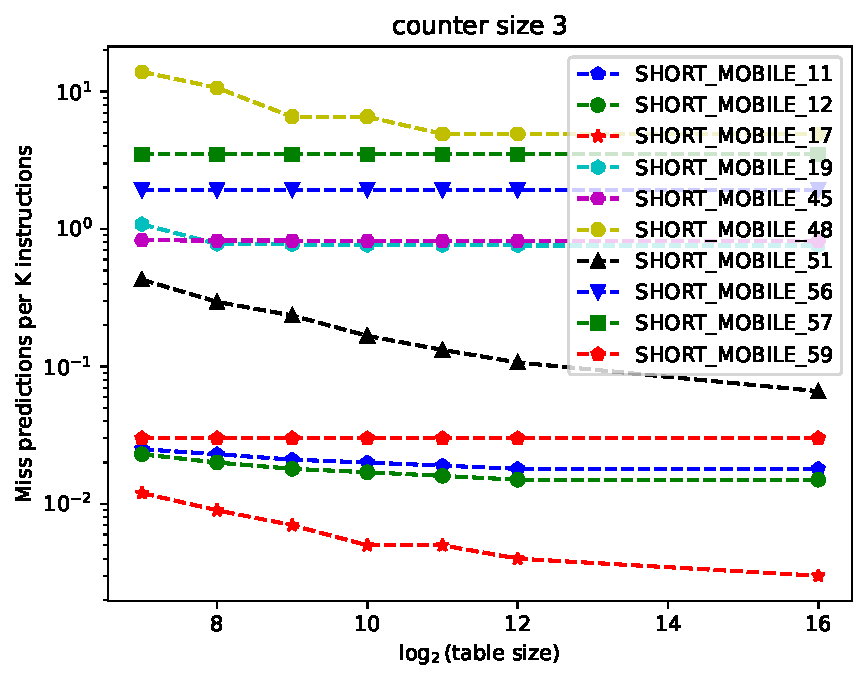
\includegraphics[width=\linewidth]{modal/graph_3_modal}
    \end{minipage}%
    \hfill
    \begin{minipage}{.48\linewidth}
    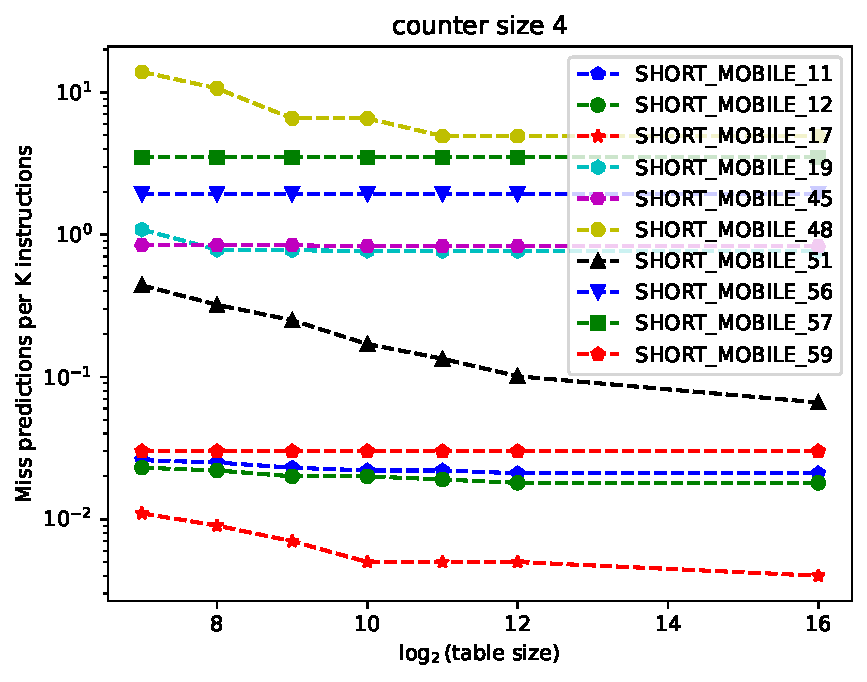
\includegraphics[width=\linewidth]{modal/graph_4_modal}
    \end{minipage}

    \begin{minipage}{.48\linewidth}
    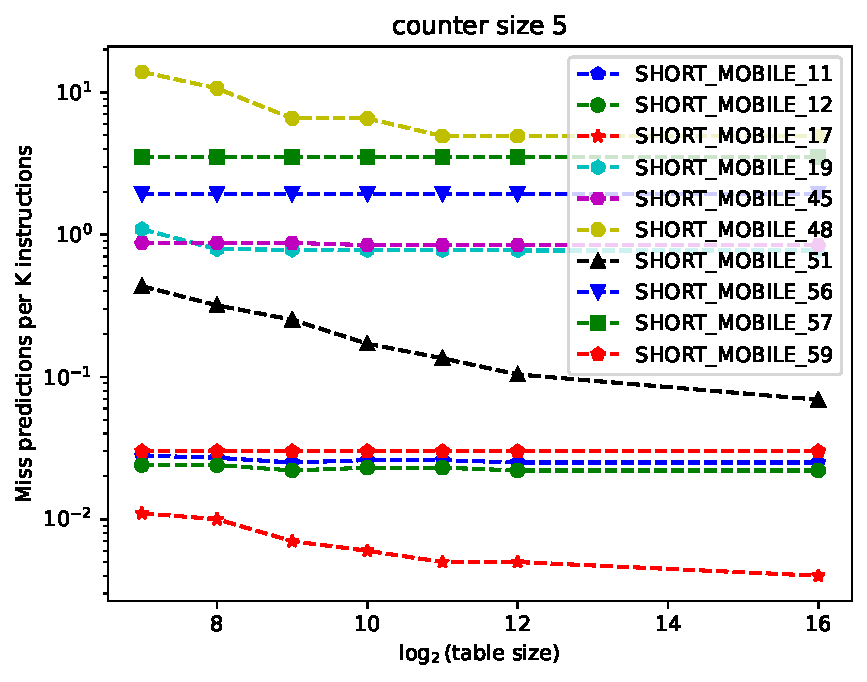
\includegraphics[width=\linewidth]{modal/graph_5_modal}
    \end{minipage}%
    \hfill
    \begin{minipage}{.48\linewidth}
    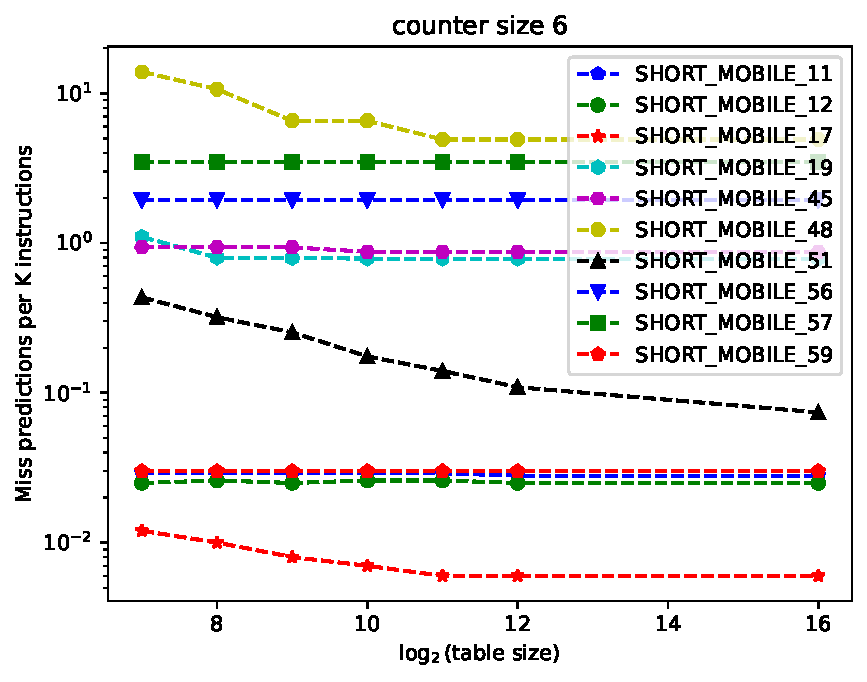
\includegraphics[width=\linewidth]{modal/graph_6_modal}
    \end{minipage}
    \subsection{Analyse}
    On voit une asymptote due à la disparition des collisions lorsque la taille du prédicteur augmente.
    Le coût du prédicteur est linéaire avec la taille du tableau, et il n'est pas raisonnable de dépasser $2^{16}$ éléments, d'autant que le gain à partir de $2^{12}$ devient très faible.
    Par ailleurs, il y a toujours moins de $7\%$ de mauvaise prédictions, ce qui est remarquable pour une approche aussi simpliste.

\clearpage
\section{Prédicteur GShare : conception et résultats}
    \subsection{Conception}
    Ce prédicteur est construit sur un historique global de $H$ bits (dans nos tests, $H = 7$) combiné à l'adresse de branchement à prédire via un XOR.
    \subsection{Résultats}
    Les résultats issus de la simulation sont les suivants.
    \par
    \begin{minipage}{.48\linewidth}
    
\includegraphics[width=\linewidth]{gshare/graph_1}
    \end{minipage}%
    \hfill
    \begin{minipage}{.48\linewidth}
    
\includegraphics[width=\linewidth]{gshare/graph_2}
    \end{minipage}

    \begin{minipage}{.48\linewidth}
    
\includegraphics[width=\linewidth]{gshare/graph_3}
    \end{minipage}%
    \hfill
    \begin{minipage}{.48\linewidth}
    
\includegraphics[width=\linewidth]{gshare/graph_4}
    \end{minipage}

    \begin{minipage}{.48\linewidth}
    
\includegraphics[width=\linewidth]{gshare/graph_5}
    \end{minipage}%
    \hfill
    \begin{minipage}{.48\linewidth}
    
\includegraphics[width=\linewidth]{gshare/graph_6}
    \end{minipage}
    \subsection{Analyse}
    On constate la même asymptote que pour le prédicteurs $n$ modal due à la disparition des collisions.
    Cependant, le taux de mauvaises prédictions est plus élevé que le prédicteur précédent pour un petit nombre d'éléments (moins de $2^{10}$). 
    Le coût du prédicteur semble exponentiel décroissant, il n'est pas non plus raisonnable de dépasser $2^{16}$ éléments car le gain à partir de $2^{12}$ devient très faible.

\clearpage
\section{Prédicteur local : conception et résultats}
    \subsection{Conception}
    Ce prédicteur utilise une table d'historique sur $H$ bits (dans nos test $H = 7$) indexée par les poids faibles de l'adresse du branchement.
    la BHT est construite sur $2^H$ bits.

    \subsection{Résultats}
    Les résultats issus de la simulation sont les suivants.
    \par
    \begin{minipage}{.48\linewidth}
    
\includegraphics[width=\linewidth]{local/graph_1}
    \end{minipage}%
    \hfill
    \begin{minipage}{.48\linewidth}
    
\includegraphics[width=\linewidth]{local/graph_2}
    \end{minipage}

    \begin{minipage}{.48\linewidth}
    
\includegraphics[width=\linewidth]{local/graph_3}
    \end{minipage}%
    \hfill
    \begin{minipage}{.48\linewidth}
    
\includegraphics[width=\linewidth]{local/graph_4}
    \end{minipage}

    \begin{minipage}{.48\linewidth}
    
\includegraphics[width=\linewidth]{local/graph_5}
    \end{minipage}%
    \hfill
    \begin{minipage}{.48\linewidth}
    
\includegraphics[width=\linewidth]{local/graph_6}
    \end{minipage}
    \subsection{Analyse}
    Les gains ne sont pas flagrants lorsque l'on augmente la taille du compteur, ce qui est logique compte tenu de la conception de la BHT qui est toujours de taille constante.
    De plus, on constate une augmentation logarithimique du taux de mauvaises prédictions jusqu'à un nombre d'élément avoisinant $2^{16}$ bits.
    Cependant, l'ensemble des mauvaises prédictions reste un petit peu bas que pour les autres prédicteurs, ce qui rend donc le prédicteur local légèrement plus efficace sur un petit nombre d'éléments.

\clearpage
\section{Métaprédicteur : conception et résultats}
    \subsection{Conception}
    Le métaprédicteur est une association des deux prédicteurs précédents qui a pour but de maximiser le taux de bonnes prédictions, avec une taille d'historique global et local de $H = 10$ bits.
    Le choix du prédicteur se fait de la manière suivante, avec une initialisation par défaut au prédicteur global :
    \begin{center}
        
\includegraphics[width=6cm]{mixte-graphe}
    \end{center}

    \subsection{Résultats}
    Les résultats issus de la simulation sont les suivants.
    \par
    \begin{minipage}{.48\linewidth}
    
\includegraphics[width=\linewidth]{meta/graph_1}
    \end{minipage}%
    \hfill
    \begin{minipage}{.48\linewidth}
    
\includegraphics[width=\linewidth]{meta/graph_2}
    \end{minipage}

    \begin{minipage}{.48\linewidth}
    
\includegraphics[width=\linewidth]{meta/graph_3}
    \end{minipage}%
    \hfill
    \begin{minipage}{.48\linewidth}
    
\includegraphics[width=\linewidth]{meta/graph_4}
    \end{minipage}

    \begin{minipage}{.48\linewidth}
    
\includegraphics[width=\linewidth]{meta/graph_5}
    \end{minipage}%
    \hfill
    \begin{minipage}{.48\linewidth}
    
\includegraphics[width=\linewidth]{meta/graph_6}
    \end{minipage}
    \subsection{Analyse}
    Il semble y avoir le comportement attendu du métaprédicteur avec les meilleures prédictions de branches de chaque prédicteur, à savoir la précision issue d'un prédicteur local pour un petit nombre d'éléments et la décroissance du taux de mauvaises prédicitons associée au prédicteur global lorsque le prédicteur local n'est pas aussi efficace.

\clearpage
\section{Perceptron : conception et résultats}
    \subsection{Conception}
    La prédiction est donnée en additionnant le produit des $n$ entrées correspondant aux bits de l'historique global de branchement (le même que pour le prédicteur gshare) et de leur poids associé.
    Au fur et à mesure des prédictions, le perceptron met à jour ses poids selon l'algorithme décrit dans le sujet de ce TP afin de devenir de plus en plus précis.

    \begin{center}
        
\includegraphics[width=12cm]{perceptron}
    \end{center}
    \clearpage

    \subsection{Résultats}
    Les résultats issus de la simulation sont les suivants.
    \par
    \begin{minipage}{.48\linewidth}
    
\includegraphics[width=\linewidth]{perceptron/graph_1}
    \end{minipage}%
    \hfill
    \begin{minipage}{.48\linewidth}
    
\includegraphics[width=\linewidth]{perceptron/graph_2}
    \end{minipage}

    \begin{minipage}{.48\linewidth}
    
\includegraphics[width=\linewidth]{perceptron/graph_3}
    \end{minipage}%
    \hfill
    \begin{minipage}{.48\linewidth}
    
\includegraphics[width=\linewidth]{perceptron/graph_4}
    \end{minipage}

    \begin{minipage}{.48\linewidth}
    
\includegraphics[width=\linewidth]{perceptron/graph_5}
    \end{minipage}%
    \hfill
    \begin{minipage}{.48\linewidth}
    
\includegraphics[width=\linewidth]{perceptron/graph_6}
    \end{minipage}
    \subsection{Analyse}
    On remarque un taux de mauvaises prédictions bien plus bas que pour les autres prédictions et cela dès $2^8$ éléments.
    On peut noter le gain flagrant d'efficacité pour chacune des traces et particulièrement la trace SHORT\_MOBILE\_48 (en jaune), qui jusque là présentait le plus haut taux de mauvaises prédiction.
    Finalement, il y a très peu d'évolution du taux de mauvaises prédictions car celui-ci reste quasi constant après $2^8$ éléments, ce qui fait du perceptron un excellent et prédicteur pour les traces qui nous ont été fournies.


\end{document}
